\documentclass[aspectratio=169,11pt]{beamer}

% ------------------------------------------------------------
% AI exposure and labor-market outcomes in Spain
% Compile with: pdflatex ai_exposure_spain_deck.tex
% ------------------------------------------------------------

\usefonttheme{professionalfonts}
\usepackage[T1]{fontenc}
\usepackage[utf8]{inputenc}
\usepackage{lmodern}
\usepackage{ragged2e}
\usepackage{graphicx}
\usepackage{booktabs}
\usepackage{amsmath,amssymb}
\usepackage{tikz}
\usepackage{array}
\usepackage{xcolor}
\usepackage{hyperref}

% Palette: warm academic policy style
\definecolor{DeepNavy}{HTML}{17324D}
\definecolor{AIRefTeal}{HTML}{0E7C7B}
\definecolor{WarmOrange}{HTML}{D95D39}
\definecolor{Gold}{HTML}{D6A738}
\definecolor{Ink}{HTML}{1F2933}
\definecolor{WarmGray}{HTML}{6B7280}
\definecolor{LightGray}{HTML}{E5E7EB}
\definecolor{Cream}{HTML}{F8F5EF}
\definecolor{SoftBlue}{HTML}{E8F1F2}
\definecolor{AlertRed}{HTML}{A23E48}
\definecolor{Forest}{HTML}{2A6F47}

\setbeamercolor{background canvas}{bg=Cream}
\setbeamercolor{normal text}{fg=Ink,bg=Cream}
\setbeamercolor{frametitle}{fg=DeepNavy,bg=Cream}
\setbeamercolor{title}{fg=DeepNavy}
\setbeamercolor{subtitle}{fg=WarmGray}
\setbeamercolor{structure}{fg=AIRefTeal}
\setbeamercolor{alerted text}{fg=AlertRed}
\setbeamercolor{footline}{fg=WarmGray,bg=Cream}

\setbeamertemplate{navigation symbols}{}
\setbeamertemplate{itemize item}{\tikz\fill[AIRefTeal] (0,0) circle (2.1pt);}
\setbeamertemplate{itemize subitem}{\tikz\fill[WarmOrange] (0,0) circle (1.5pt);}
\setbeamertemplate{frametitle}{%
  \vspace{0.45cm}%
  \begin{tikzpicture}[remember picture,overlay]
    \fill[AIRefTeal] (current page.north west) ++(0.55cm,-0.55cm) rectangle ++(0.08cm,-0.62cm);
  \end{tikzpicture}%
  \hspace{0.45cm}\insertframetitle\par\vspace{0.16cm}
}
\setbeamertemplate{footline}{%
  \hfill\scriptsize\insertframenumber\,/\,\inserttotalframenumber\hspace{0.4cm}\vspace{0.25cm}
}

\newcommand{\bigclaim}[1]{%
  \begin{center}\Large\bfseries\color{DeepNavy}#1\end{center}
}
\newcommand{\smallnote}[1]{\vspace{0.1cm}{\scriptsize\color{WarmGray}#1}}
\newcommand{\highlightnum}[2]{%
  \begin{tikzpicture}
    \node[rounded corners=3pt, fill=SoftBlue, draw=AIRefTeal, line width=0.7pt, inner sep=5pt] {\begin{minipage}{#1}\centering #2\end{minipage}};
  \end{tikzpicture}
}
\newcommand{\transitionslide}[2]{%
  \begin{frame}[plain]
    \begin{tikzpicture}[remember picture,overlay]
      \fill[DeepNavy] (current page.south west) rectangle (current page.north east);
      \node[align=center, text=white, font=\Huge\bfseries, text width=0.82\paperwidth] at (current page.center) {#1};
      \node[align=center, text=Gold, font=\large, text width=0.78\paperwidth] at ([yshift=-1.25cm]current page.center) {#2};
    \end{tikzpicture}
  \end{frame}
}

\title{AI Exposure and Labor-Market Outcomes in Spain}
\subtitle{Suggestive divergence, fragile identification, and the next empirical steps}
\author{Unknown}
\institute{AIReF}
\date{June 2026}

\begin{document}
\RaggedRight

% 1
\begin{frame}[plain]
  \begin{tikzpicture}[remember picture,overlay]
    \fill[Cream] (current page.south west) rectangle (current page.north east);
    \fill[DeepNavy] (current page.south west) rectangle ([xshift=4.6cm]current page.north west);
    \node[anchor=west, text=white, font=\Large\bfseries, text width=3.55cm] at ([xshift=0.65cm,yshift=-2.0cm]current page.north west) {AI exposure\\meets Spanish labor markets};
    \node[anchor=west, text=DeepNavy, font=\huge\bfseries, text width=9.0cm] at ([xshift=5.25cm,yshift=-2.0cm]current page.north west) {AI Exposure and Labor-Market Outcomes in Spain};
    \node[anchor=west, text=WarmGray, font=\large, text width=8.8cm] at ([xshift=5.25cm,yshift=-3.55cm]current page.north west) {A research memo distilled into a 10--15 slide academic presentation};
    \node[anchor=west, text=Ink, font=\normalsize] at ([xshift=5.25cm,yshift=-5.1cm]current page.north west) {Unknown \hspace{0.25cm}\textbar\hspace{0.25cm} AIReF \hspace{0.25cm}\textbar\hspace{0.25cm} June 2026};
  \end{tikzpicture}
\end{frame}

% 2
\begin{frame}{The key question is not whether exposed jobs changed; it is whether AI caused the change}
  \vspace{0.25cm}
  \begin{columns}[T,onlytextwidth]
    \column{0.48\textwidth}
      \highlightnum{0.88\linewidth}{\Large Spanish CNO4 occupations\\[0.1cm]\normalsize matched to semantic AI exposure}
      \vspace{0.5cm}
      \highlightnum{0.88\linewidth}{\Large Monthly SEPE panel\\[0.1cm]\normalsize January 2021--March 2026}
    \column{0.48\textwidth}
      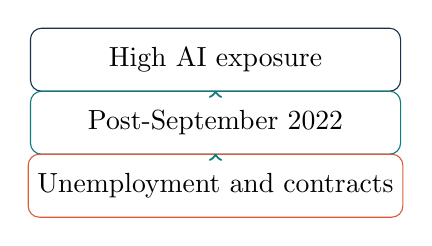
\begin{tikzpicture}[node distance=0.8cm]
        \node[draw=DeepNavy, rounded corners, fill=white, minimum width=4.7cm, minimum height=0.8cm, align=center] (a) {High AI exposure};
        \node[draw=AIRefTeal, rounded corners, fill=white, minimum width=4.7cm, minimum height=0.8cm, below of=a, align=center] (b) {Post-September 2022};
        \node[draw=WarmOrange, rounded corners, fill=white, minimum width=4.7cm, minimum height=0.8cm, below of=b, align=center] (c) {Unemployment and contracts};
        \draw[->, thick, AIRefTeal] (a) -- (b);
        \draw[->, thick, AIRefTeal] (b) -- (c);
      \end{tikzpicture}
      \vspace{0.35cm}

      \small The empirical task is to separate a post-2022 occupational divergence from broader family-level shocks, churn, and reallocation.
  \end{columns}
\end{frame}

% 3
\begin{frame}{High-exposure occupations diverge after 2022 in registered unemployment}
  \centering
  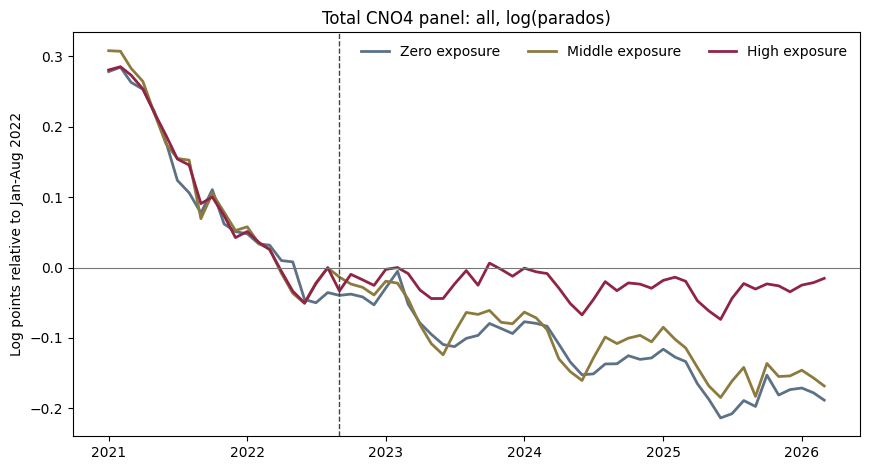
\includegraphics[width=0.82\linewidth,height=0.68\textheight,keepaspectratio]{figures/figure_memo_v2_indexed_total_all_ln_parados.png}

  \smallnote{Indexed paths use the January--August 2022 mean as the normalization window. The figure is descriptive, not causal.}
\end{frame}

% 4
\begin{frame}{Contracts also rise, so the simple displacement story is incomplete}
  \centering
  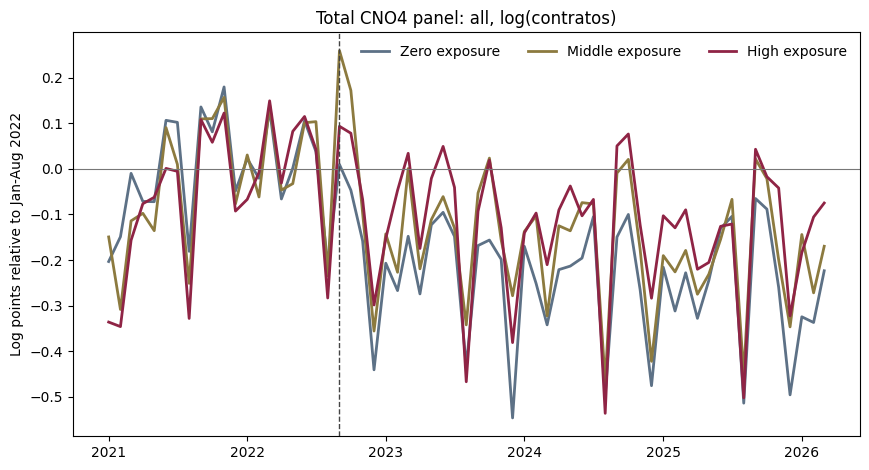
\includegraphics[width=0.82\linewidth,height=0.68\textheight,keepaspectratio]{figures/figure_memo_v2_indexed_total_all_ln_contratos.png}

  \smallnote{A rise in contracts in high-exposure occupations points toward churn, reallocation, or composition changes, not only lower labor demand.}
\end{frame}

% 5
\begin{frame}{The exposure measure is rich, but it is potential exposure rather than observed adoption}
  \begin{columns}[T,onlytextwidth]
    \column{0.54\textwidth}
      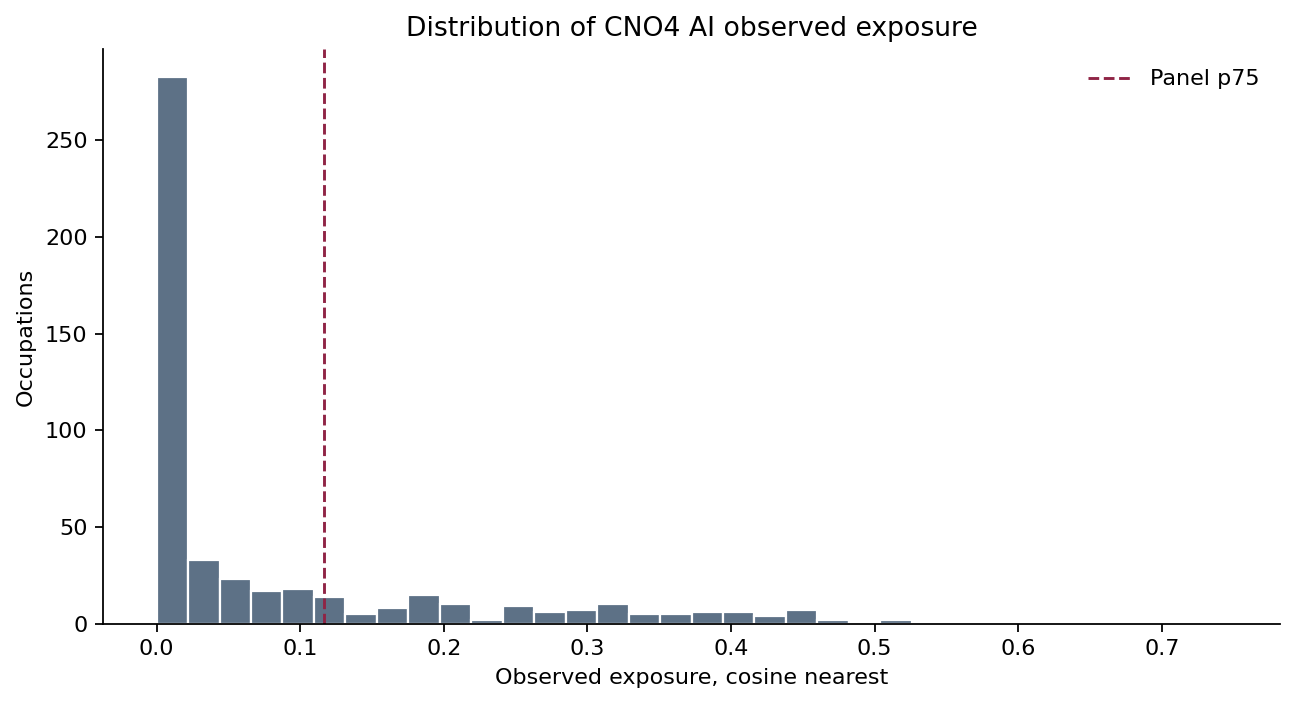
\includegraphics[width=\linewidth,height=0.64\textheight,keepaspectratio]{figures/figure_03_exposure_distribution.png}
    \column{0.42\textwidth}
      \vspace{0.4cm}
      \begin{itemize}
        \item Time-invariant CNO4 semantic exposure.
        \item Based on Spanish adaptation of Anthropic/O*NET exposure concepts.
        \item Best interpreted as task exposure, not monthly firm-level AI use.
      \end{itemize}
      \vspace{0.35cm}
      \alert{Implication:} the design tests whether exposed occupations moved differently after diffusion, not who adopted AI.
  \end{columns}
\end{frame}

% 6
\begin{frame}{The baseline TWFE estimate is positive and economically visible}
  \begin{columns}[T,onlytextwidth]
    \column{0.44\textwidth}
      \vspace{0.35cm}
      \highlightnum{0.95\linewidth}{\Huge 0.089\\[-0.05cm]\normalsize log points in registered unemployment}
      \vspace{0.35cm}
      \highlightnum{0.95\linewidth}{\Huge +9.3\%\\[-0.05cm]\normalsize approximate post-2022 relative increase}
    \column{0.52\textwidth}
      \vspace{0.25cm}
      \begin{equation*}
      y_{ot}=\alpha_o+\lambda_t+\beta\left(HighAI_o\times Post_t\right)+\varepsilon_{ot}
      \end{equation*}
      \vspace{0.25cm}
      \small
      The coefficient compares high-exposure CNO4 occupations with zero-exposure occupations after September 2022, absorbing occupation and month fixed effects.
  \end{columns}
\end{frame}

% 7
\begin{frame}{The baseline event study fails the parallel-trends test}
  \centering
  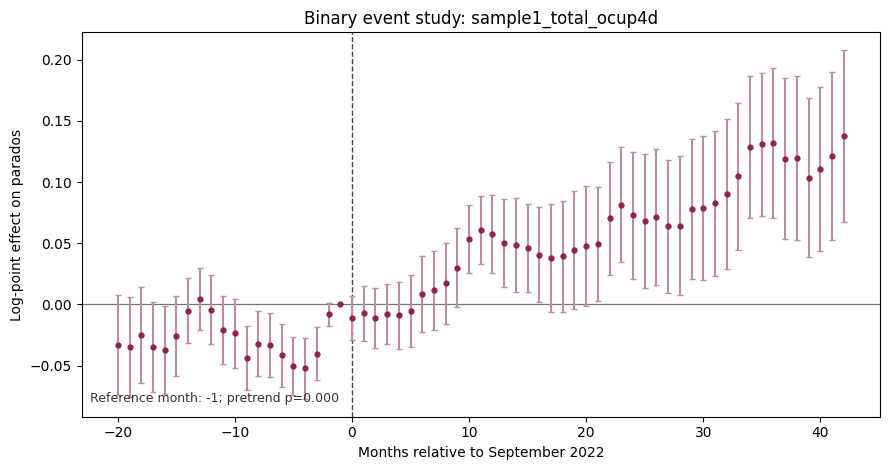
\includegraphics[width=0.82\linewidth,height=0.70\textheight,keepaspectratio]{figures/figure_binary_event_study_sample1_total_ocup4d.png}

  \smallnote{This is the central reason not to present the baseline TWFE coefficient as causal.}
\end{frame}

% 8
\begin{frame}{Within-CNO2 comparisons are cleaner, but the identifying variation becomes thin}
  \begin{columns}[T,onlytextwidth]
    \column{0.50\textwidth}
      \centering
      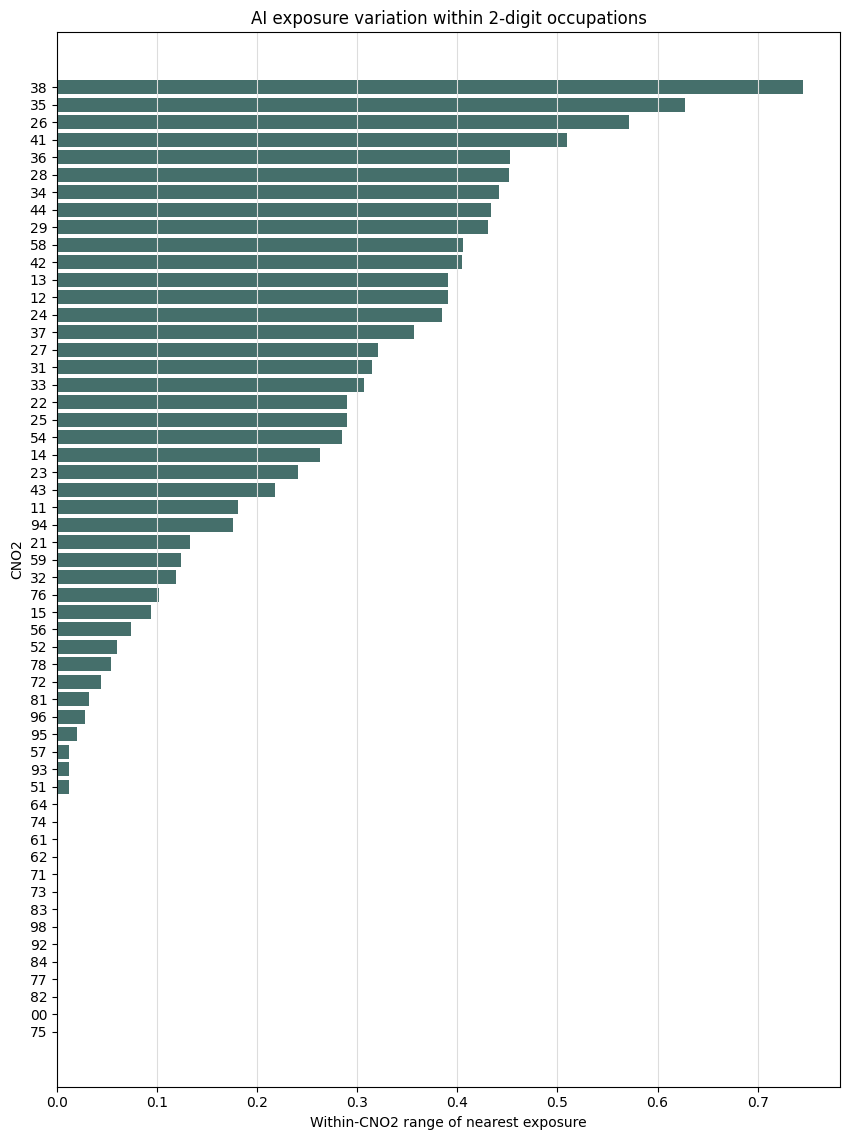
\includegraphics[width=0.82\linewidth,height=0.68\textheight,keepaspectratio]{figures/figure_exposure_variation_within_cno2.png}
    \column{0.46\textwidth}
      \vspace{0.35cm}
      \small
      CNO2-by-month fixed effects compare detailed occupations within the same broad occupational family and month.
      \vspace{0.35cm}
      \begin{itemize}
        \item This is conceptually attractive.
        \item It discards between-family variation.
        \item Power depends on within-family exposure support.
      \end{itemize}
      \vspace{0.2cm}
      \alert{Interpretation:} imprecision is not proof of zero effect; it shows the baseline depends heavily on broad occupational-family dynamics.
  \end{columns}
\end{frame}

% 9
\begin{frame}{Continuous DiD uses the full exposure dose instead of a high-versus-zero cutoff}
  \centering
  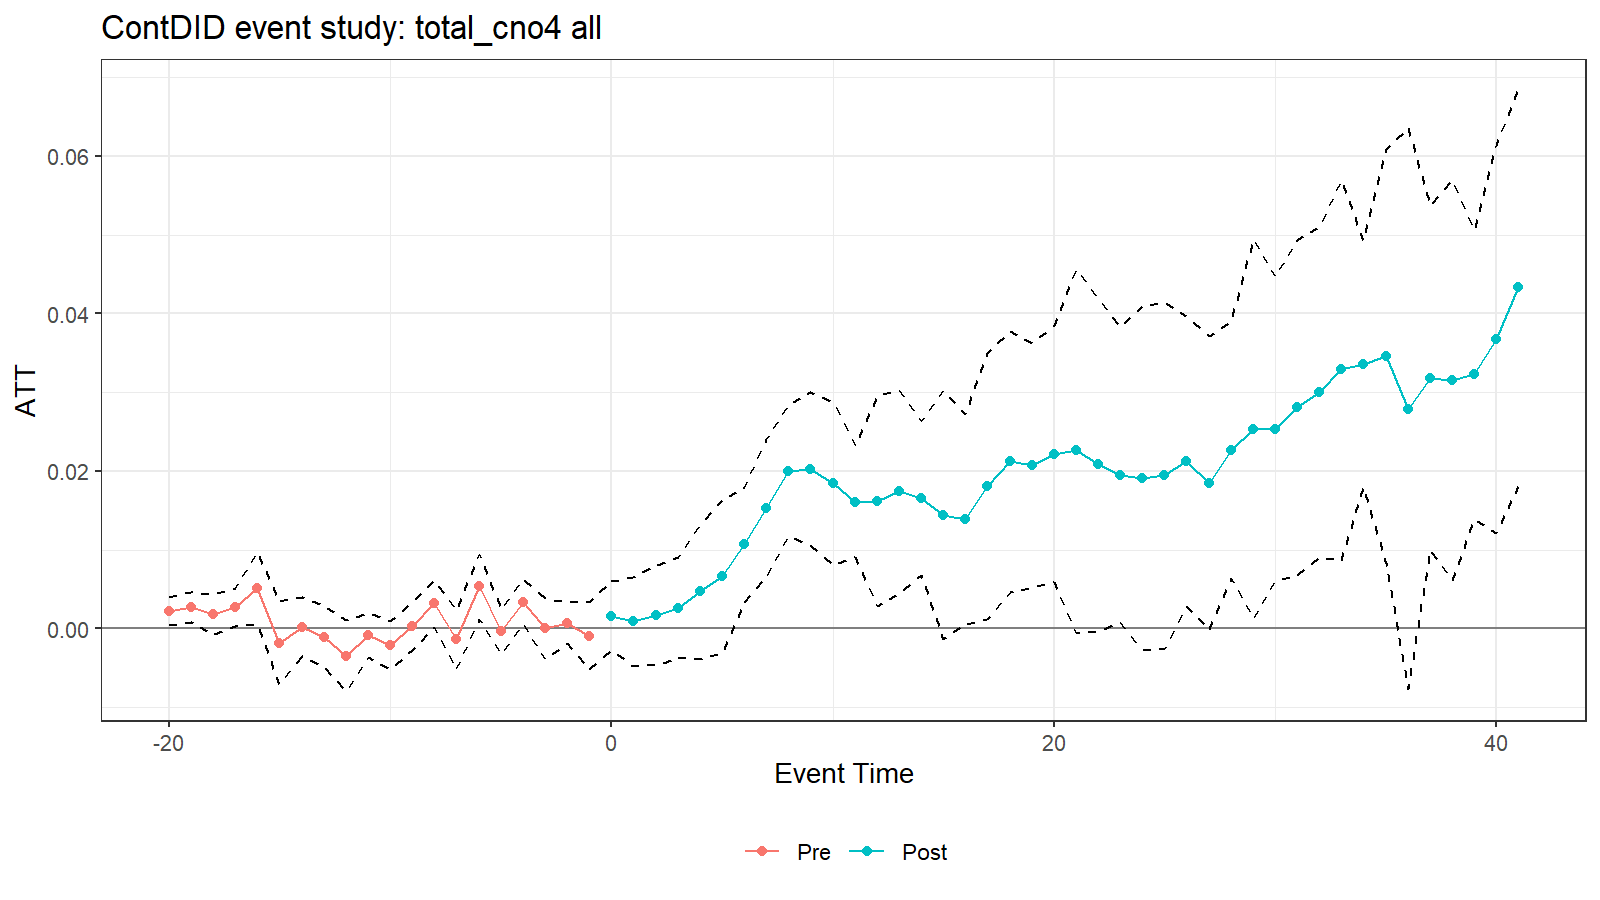
\includegraphics[width=0.86\linewidth,height=0.70\textheight,keepaspectratio]{figures/figure_contdid_eventstudy_total_cno4_all.png}

  \smallnote{The contdid estimator is useful because it asks whether outcomes vary smoothly with the continuous exposure measure.}
\end{frame}

% 10
\begin{frame}{The dose-response pattern is suggestive, but support and functional-form checks matter}
  \centering
  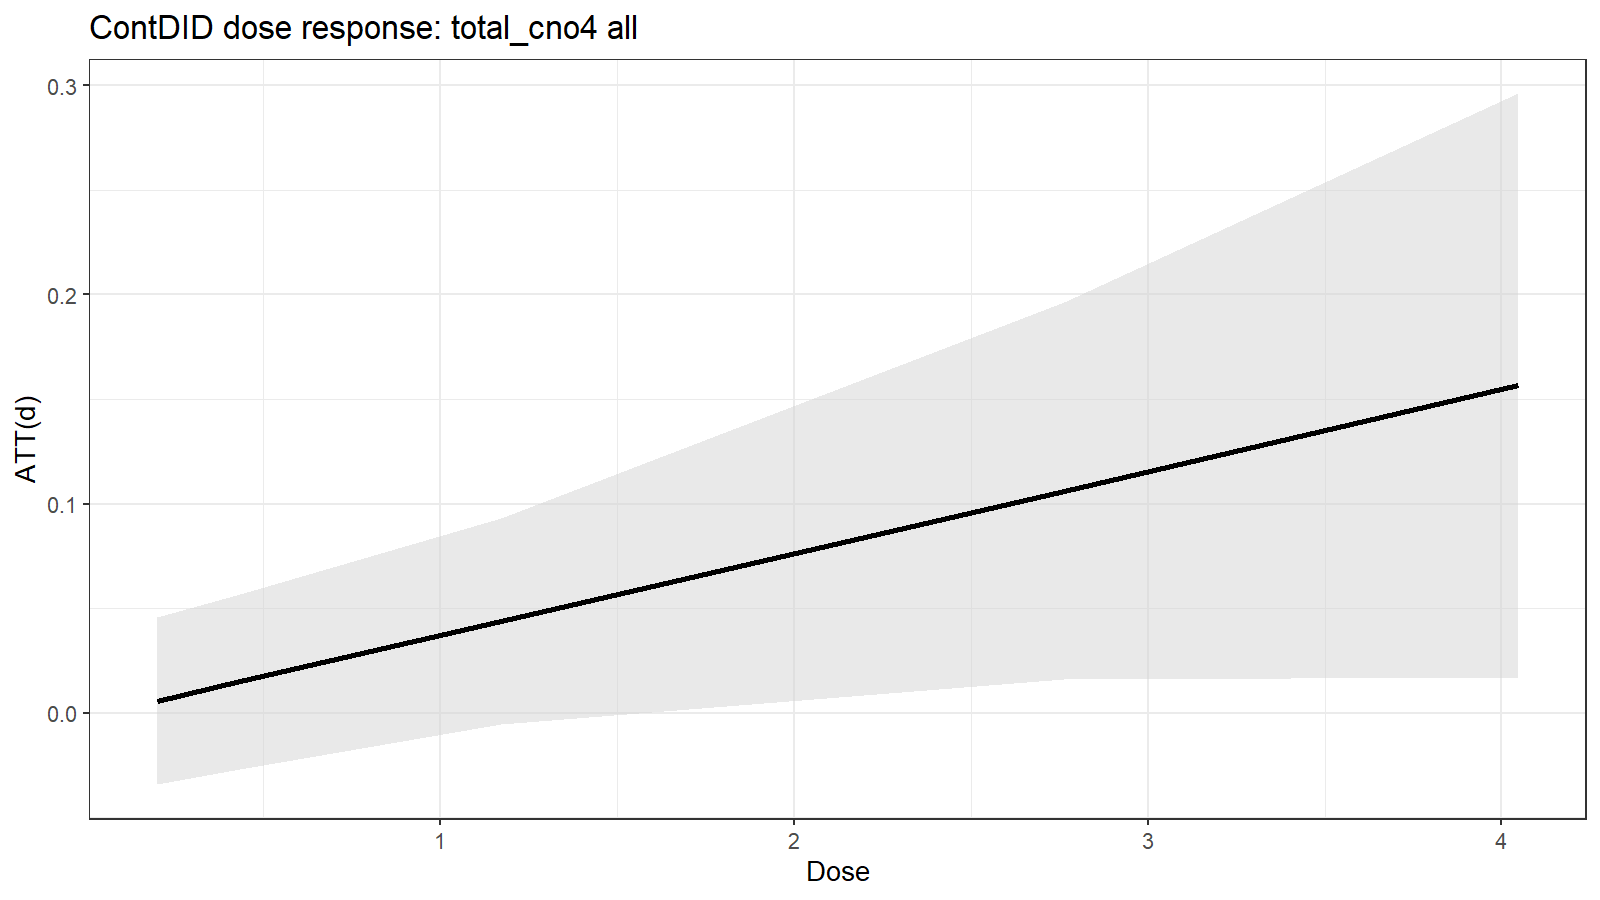
\includegraphics[width=0.86\linewidth,height=0.70\textheight,keepaspectratio]{figures/figure_contdid_dose_response_total_cno4_all.png}

  \smallnote{A dose-response plot is persuasive only where the exposure distribution has adequate support and pre-period balance is credible.}
\end{frame}

% 11
\begin{frame}{Synthetic DiD asks whether donors can reproduce the treated pre-period path}
  \begin{columns}[T,onlytextwidth]
    \column{0.56\textwidth}
      \centering
      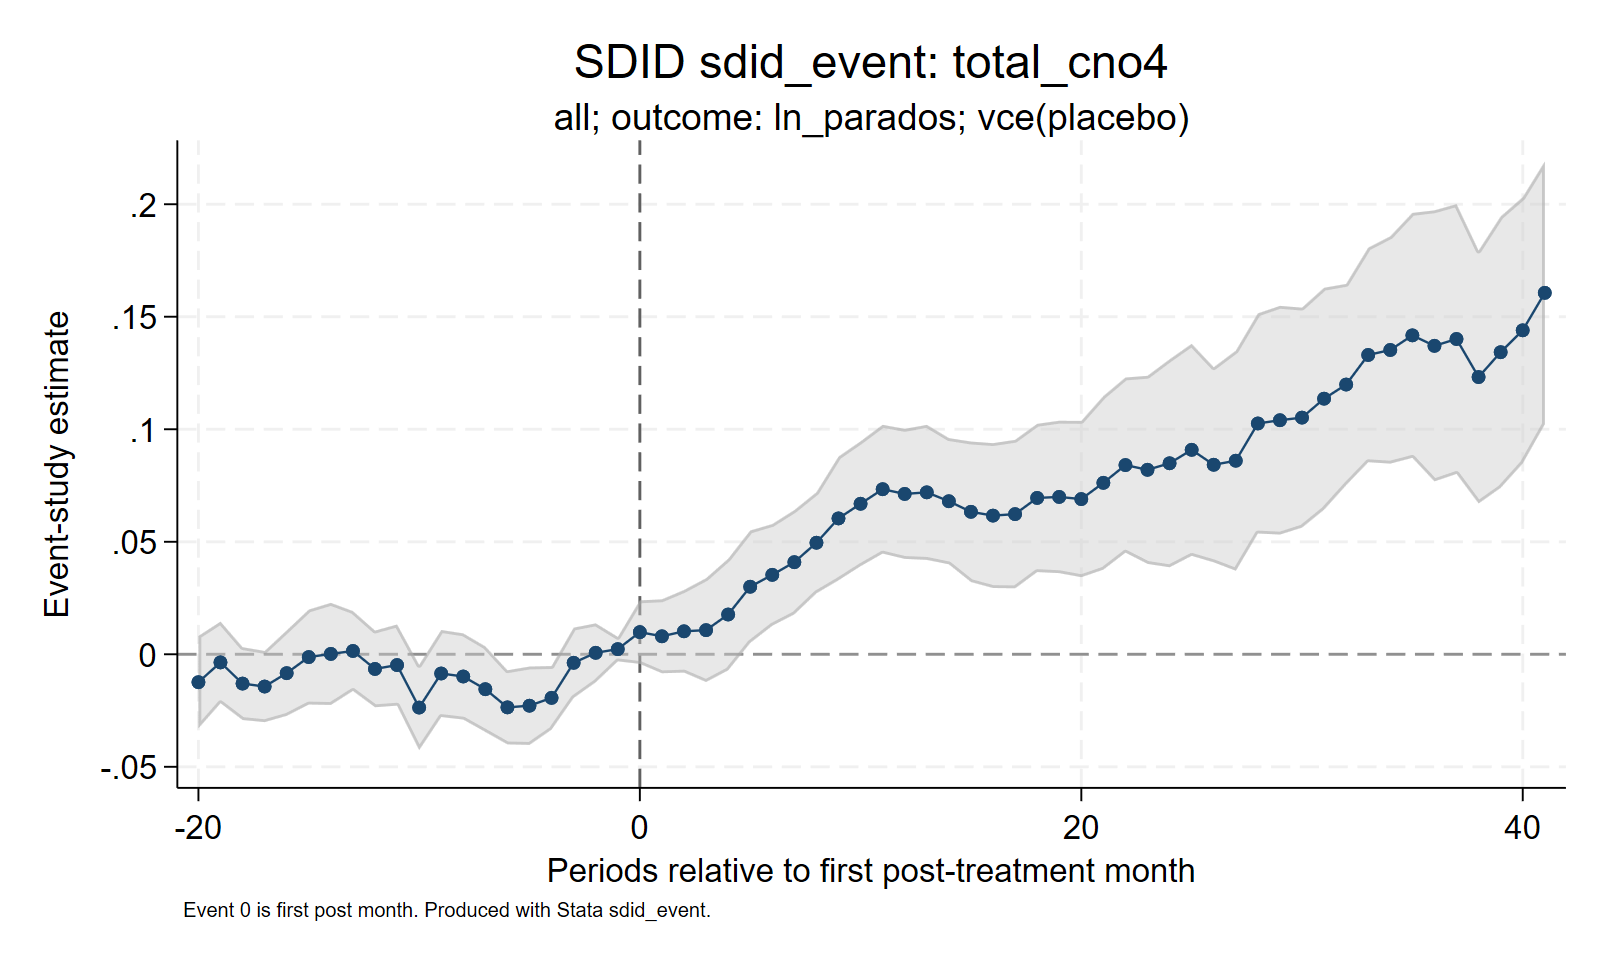
\includegraphics[width=\linewidth,height=0.66\textheight,keepaspectratio]{figures/sdid_event_focused_sdid_total_cno4_ln_parados.png}
    \column{0.40\textwidth}
      \vspace{0.45cm}
      \small
      SDID is the right complement after TWFE pretrend failures because it forces the control group to look like the treated group before the diffusion window.
      \vspace{0.35cm}
      \begin{itemize}
        \item Check pre-period fit.
        \item Inspect donor weights.
        \item Test sensitivity to donor pool restrictions.
      \end{itemize}
  \end{columns}
\end{frame}

% 12
\begin{frame}{Age heterogeneity points to the 30--39 group, but the result needs discipline}
  \begin{columns}[T,onlytextwidth]
    \column{0.49\textwidth}
      \centering
      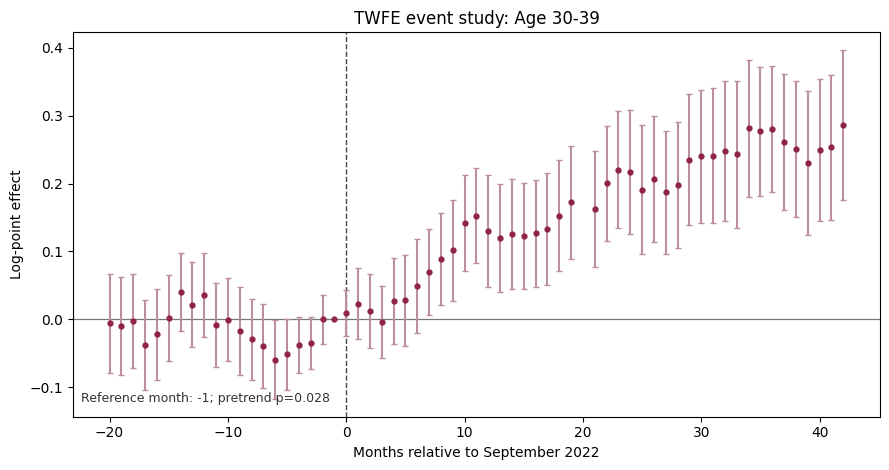
\includegraphics[width=\linewidth,height=0.60\textheight,keepaspectratio]{figures/figure_memo_v2_twfe_event_age3_30_39.png}
      \small TWFE event study
    \column{0.49\textwidth}
      \centering
      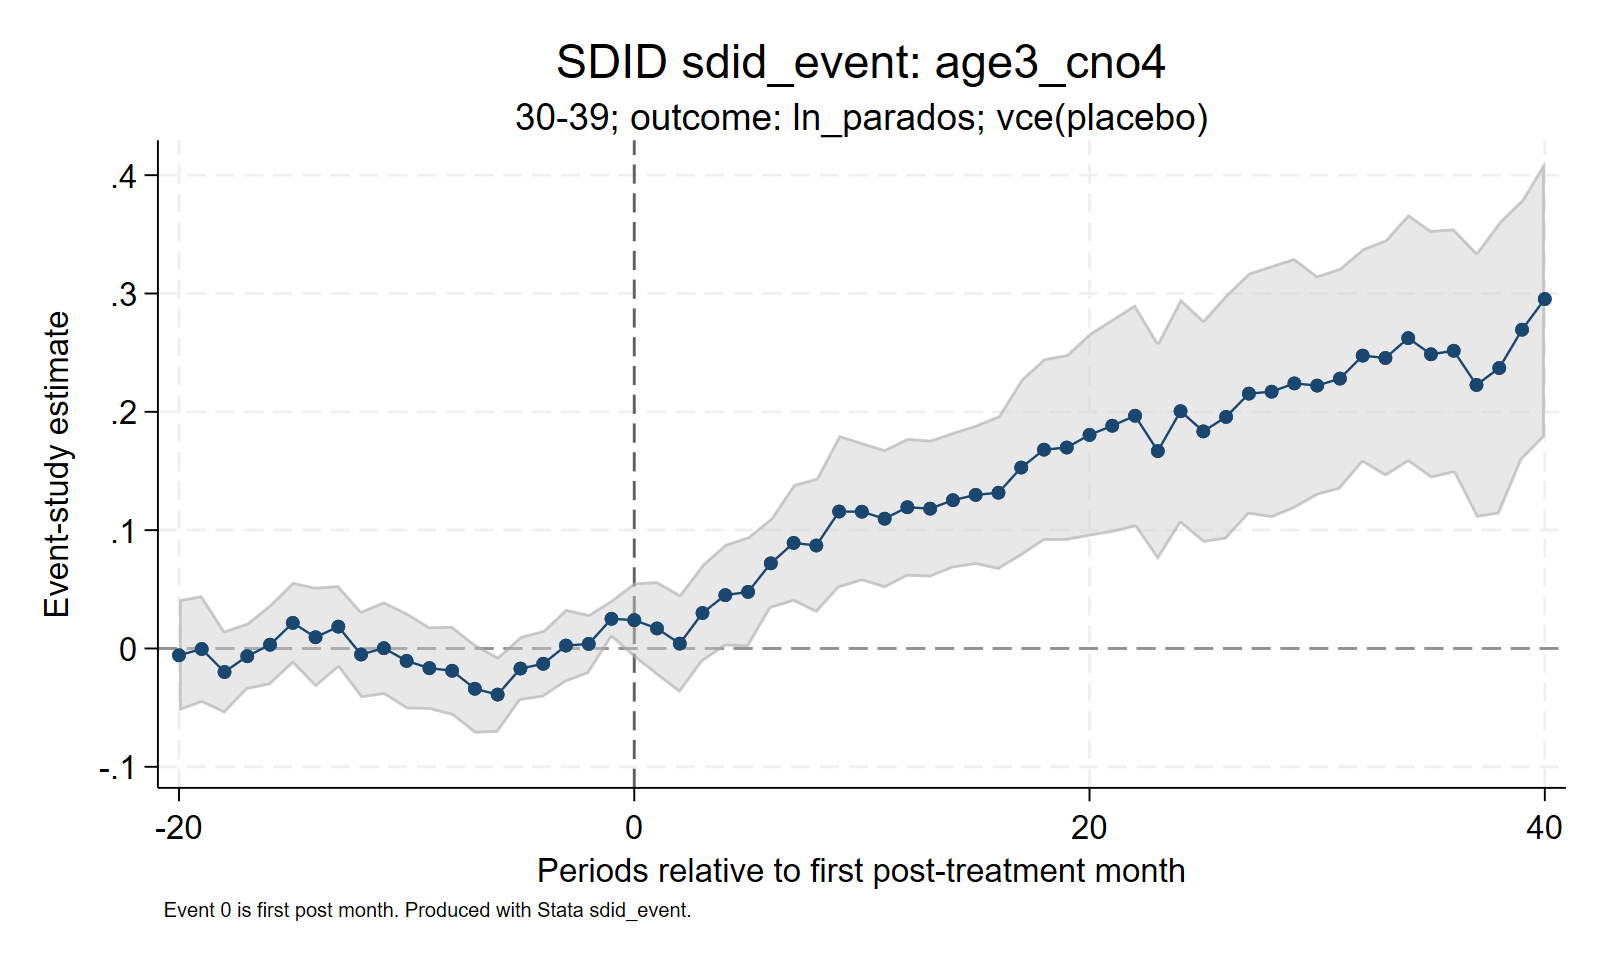
\includegraphics[width=\linewidth,height=0.60\textheight,keepaspectratio]{figures/sdid_event_focused_sdid_age3_30_39_ln_parados.png}
      \small SDID event study
  \end{columns}
  \smallnote{Treat this as a priority robustness target, not as a standalone causal claim.}
\end{frame}

% 13
\begin{frame}{HonestDiD-style sensitivity should decide how much weight to put on the TWFE event study}
  \centering
  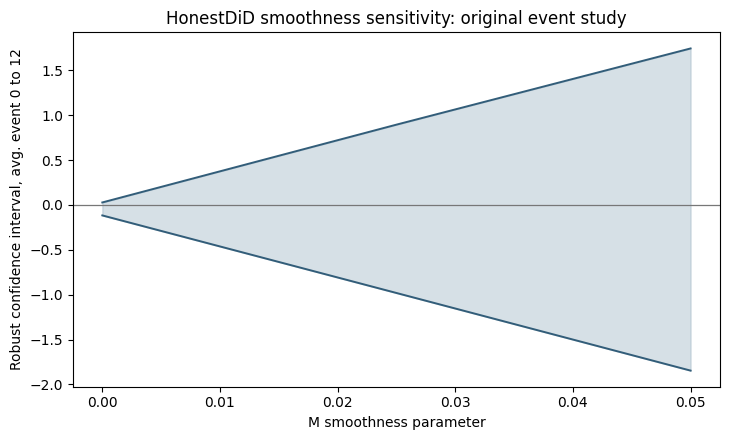
\includegraphics[width=0.74\linewidth,height=0.64\textheight,keepaspectratio]{figures/figure_09_recommended_honestdid_smoothness_original.png}

  \smallnote{Sensitivity analysis is especially important because the identifying assumptions are visibly strained in the baseline event study.}
\end{frame}

% 14
\begin{frame}{The most defensible conclusion is conservative}
  \vspace{0.2cm}
  \bigclaim{High-AI-exposure occupations show a positive post-2022 divergence, but the current evidence does not yet establish that AI exposure caused higher unemployment.}
  \vspace{0.35cm}
  \begin{columns}[T,onlytextwidth]
    \column{0.31\textwidth}
      \highlightnum{0.95\linewidth}{\bfseries What is robust?\\[0.1cm]\small A descriptive post-2022 divergence in high-exposure occupations.}
    \column{0.31\textwidth}
      \highlightnum{0.95\linewidth}{\bfseries What is fragile?\\[0.1cm]\small Parallel trends and between-family occupational dynamics.}
    \column{0.31\textwidth}
      \highlightnum{0.95\linewidth}{\bfseries What comes next?\\[0.1cm]\small ContDID, SDID, support diagnostics, and donor-weight audits.}
  \end{columns}
\end{frame}

% 15
\begin{frame}[plain]
  \begin{tikzpicture}[remember picture,overlay]
    \fill[DeepNavy] (current page.south west) rectangle (current page.north east);
    \node[align=center, text=white, font=\Huge\bfseries, text width=0.84\paperwidth] at ([yshift=0.25cm]current page.center) {The evidence is strongest as a warning signal, not yet as a causal verdict.};
    \node[align=center, text=Gold, font=\Large, text width=0.78\paperwidth] at ([yshift=-1.45cm]current page.center) {The next version should make identification, not estimation, the center of the paper.};
  \end{tikzpicture}
\end{frame}

\end{document}
